\documentclass{article}

\usepackage[french]{babel}
\usepackage[utf8]{inputenc}
\usepackage[T1]{fontenc}
\usepackage{verbatim}
\usepackage{amsmath}
\usepackage{geometry}
\usepackage{graphicx}

\usepackage[final]{pdfpages}

%% Si ca ne compile pas chez vous, mettez la ligne suivante en commentaire
%\usepackage{tikz}

\date{\vspace{3 cm} \today}
\author{\vspace{4 cm} \\ Groupe :\\ \\Ben Brahim Dhouha\\Meunier Bastien\\Wang Miao }
\title{Rapport du projet SGBD \\ Gestion d'un club sportif}


\usepackage{fancyhdr}
\lhead{Projet SGBD du semestre S7 - Basket-ball }
\rhead{}
\renewcommand{\headrulewidth}{1px}
\lfoot{ \bsc{Enseirb-Matmeca 2012-2013}}
\rfoot{ \bsc{Filière Informatique - I2}}
\renewcommand{\footrulewidth}{1px}
\pagestyle{fancy}


\begin{document}

\thispagestyle{empty}
\begin{figure}

\includegraphics[width=0.25\textwidth]{enseirb-matmeca.png}
\end{figure}
\maketitle

\newpage

\section*{Introduction}

Afin de garder les information sur ses membres et sur son foncionnement, un club sportif peut être amener à utiliser une base de données. Ce projet consite en l'implémentation d'une base de données pour un club de basket-ball gérant les rencontres entre les différents clubs d'une fédération. \\

Dans ce rapport, il sera question, en premier temps, de présenter le modèle conceptuel utilisé pour la modélisation des données, puis le modèle relationnel en $3^{ème}$ forme normale. Ensuite, l'implémentation de la base en MySQL ainsi que la justification de notre choix. Enfin, l'environnement d'exécution avec un apercu de l'interface graphique concue pour accéder à la base. 

%Ainsi, nous avons dû créer deux fichiers afin de créer la base : base.sql et données.sql qui nous ont ensuite servi à tester nos requêtes.
%Puis, nous avons créer les requêtes et enfin l'interface graphique permettant leur utilisation. Pour celle-ci nous avons choisi jdbc car nous avons une bonne maîtrise du java.

\newpage
\tableofcontents

\newpage
\section{Modèle conceptuel}

\subsection{Description du contexte de l'application}
Pour la modélisation conceptuelle des données nous avons créé au départ 6 entités : \\


\begin{itemize}
\item entité \textit{Club} dans laquelle nous avons stocké le numéro identifiant et le nom du club.
\item entité \textit{Bureau} contenant son numéro ainsi que les noms du président, vice-président et trésorier. 
\item entité \textit{Equipe} contenant le numéro et le nom de l'équipe.
\item entité \textit{Catégorie} contenant le numéro et le nom de la catégorie (junior, cadet, benjamen, etc )
\item entité \textit{Joueur} contenant le numéro de licence du joueur ainsi que son nom, son prénom, sa date de naissance, son adresse, sa date d'entrée dans le club, les cumuls des points marqués et des fautes.
\item entité \textit{Entraîneur} contenant le numéro identifiant de l'entraîneur ainsi que son nom, son prénom et sa date d'entrée dans le club. \\
\end{itemize}



Dans un premier temps nous avons choisi de modéliser les rencontres entre par une association entre deux équipes et dans laquelle on stocke le score et la date de la rencontre. Nous nous sommes rendus compte par la suite qu une telle modélisation pose quelques problèmes : d'une part, on ne peut pas savoir quel joueur a participé à quelle rencontre. D'autre part, il nous est impossible de savoir quel joueur a marqué dans quelle rencontre ce qui pose un problème pour le calcul des cumuls des points marqués et des fautes pour chaque joueur ou même encore au niveau des statistiques notamment au niveau du classement des meilleurs joueurs d'une journée pour une catégorie. Nous avons donc crée une entité \textit{Rencontre} dans laquelle on stocke le numéro de la rencontre ainsi que le score et la date. De cette manière, un joueur peut jouer à différentes rencontres.
\\

Un nouveau problème s'est posé par la suite lors de l'implémentation de la base. Le modèle choisi a entraîné une énorme duplication de données au niveau de la table des joueurs. Etant donnée que les joueurs peuvent participer à plusieurs rencontres, nous devons à chaque fois réinsérer le nom, le prénom, le numéro de licence, sa date de naissance, son adresse et sa date d'entrée dans le club pour chaque match joué rien que pour stocker le nombre de points marqués et des fautes. La solution était donc d'enlever ces deux derniers attributs et de les insérer dans l'assocation \textit{participe} qui relie le joueur et la rencontre puisqu'ils dépendent de ces deux entités. Cela nous a permis d'éviter la duplication des données.
\\


Le dernier problème rencontré concernait les membres du bureau. Comme il est précedemment expliqué, nous avons créer une entité \textit{Bureau} qui a pour attribut -entre autres- les noms du président, du vice-président et du trésorier. Cela nous empêchait de stocker d'autres informations concernant les membres du bureau notamment le prénom, la date de naissance ou encore le numéro identifiant. L'idée était d'ajouter une nouvelle entité \textit{Membre du bureau} permettant de stocker ces informations. L'entité \textit{Bureau} ne contenant plus que le numéro du bureau et ayant une association 1,1 des deux côtés avec le club devient alors inutile.  


\newpage


\subsection{Schéma entité-association }
Après différentes modifications, voici le schéma entité-association :
 
\begin{figure}
\includegraphics{}
\end{figure}

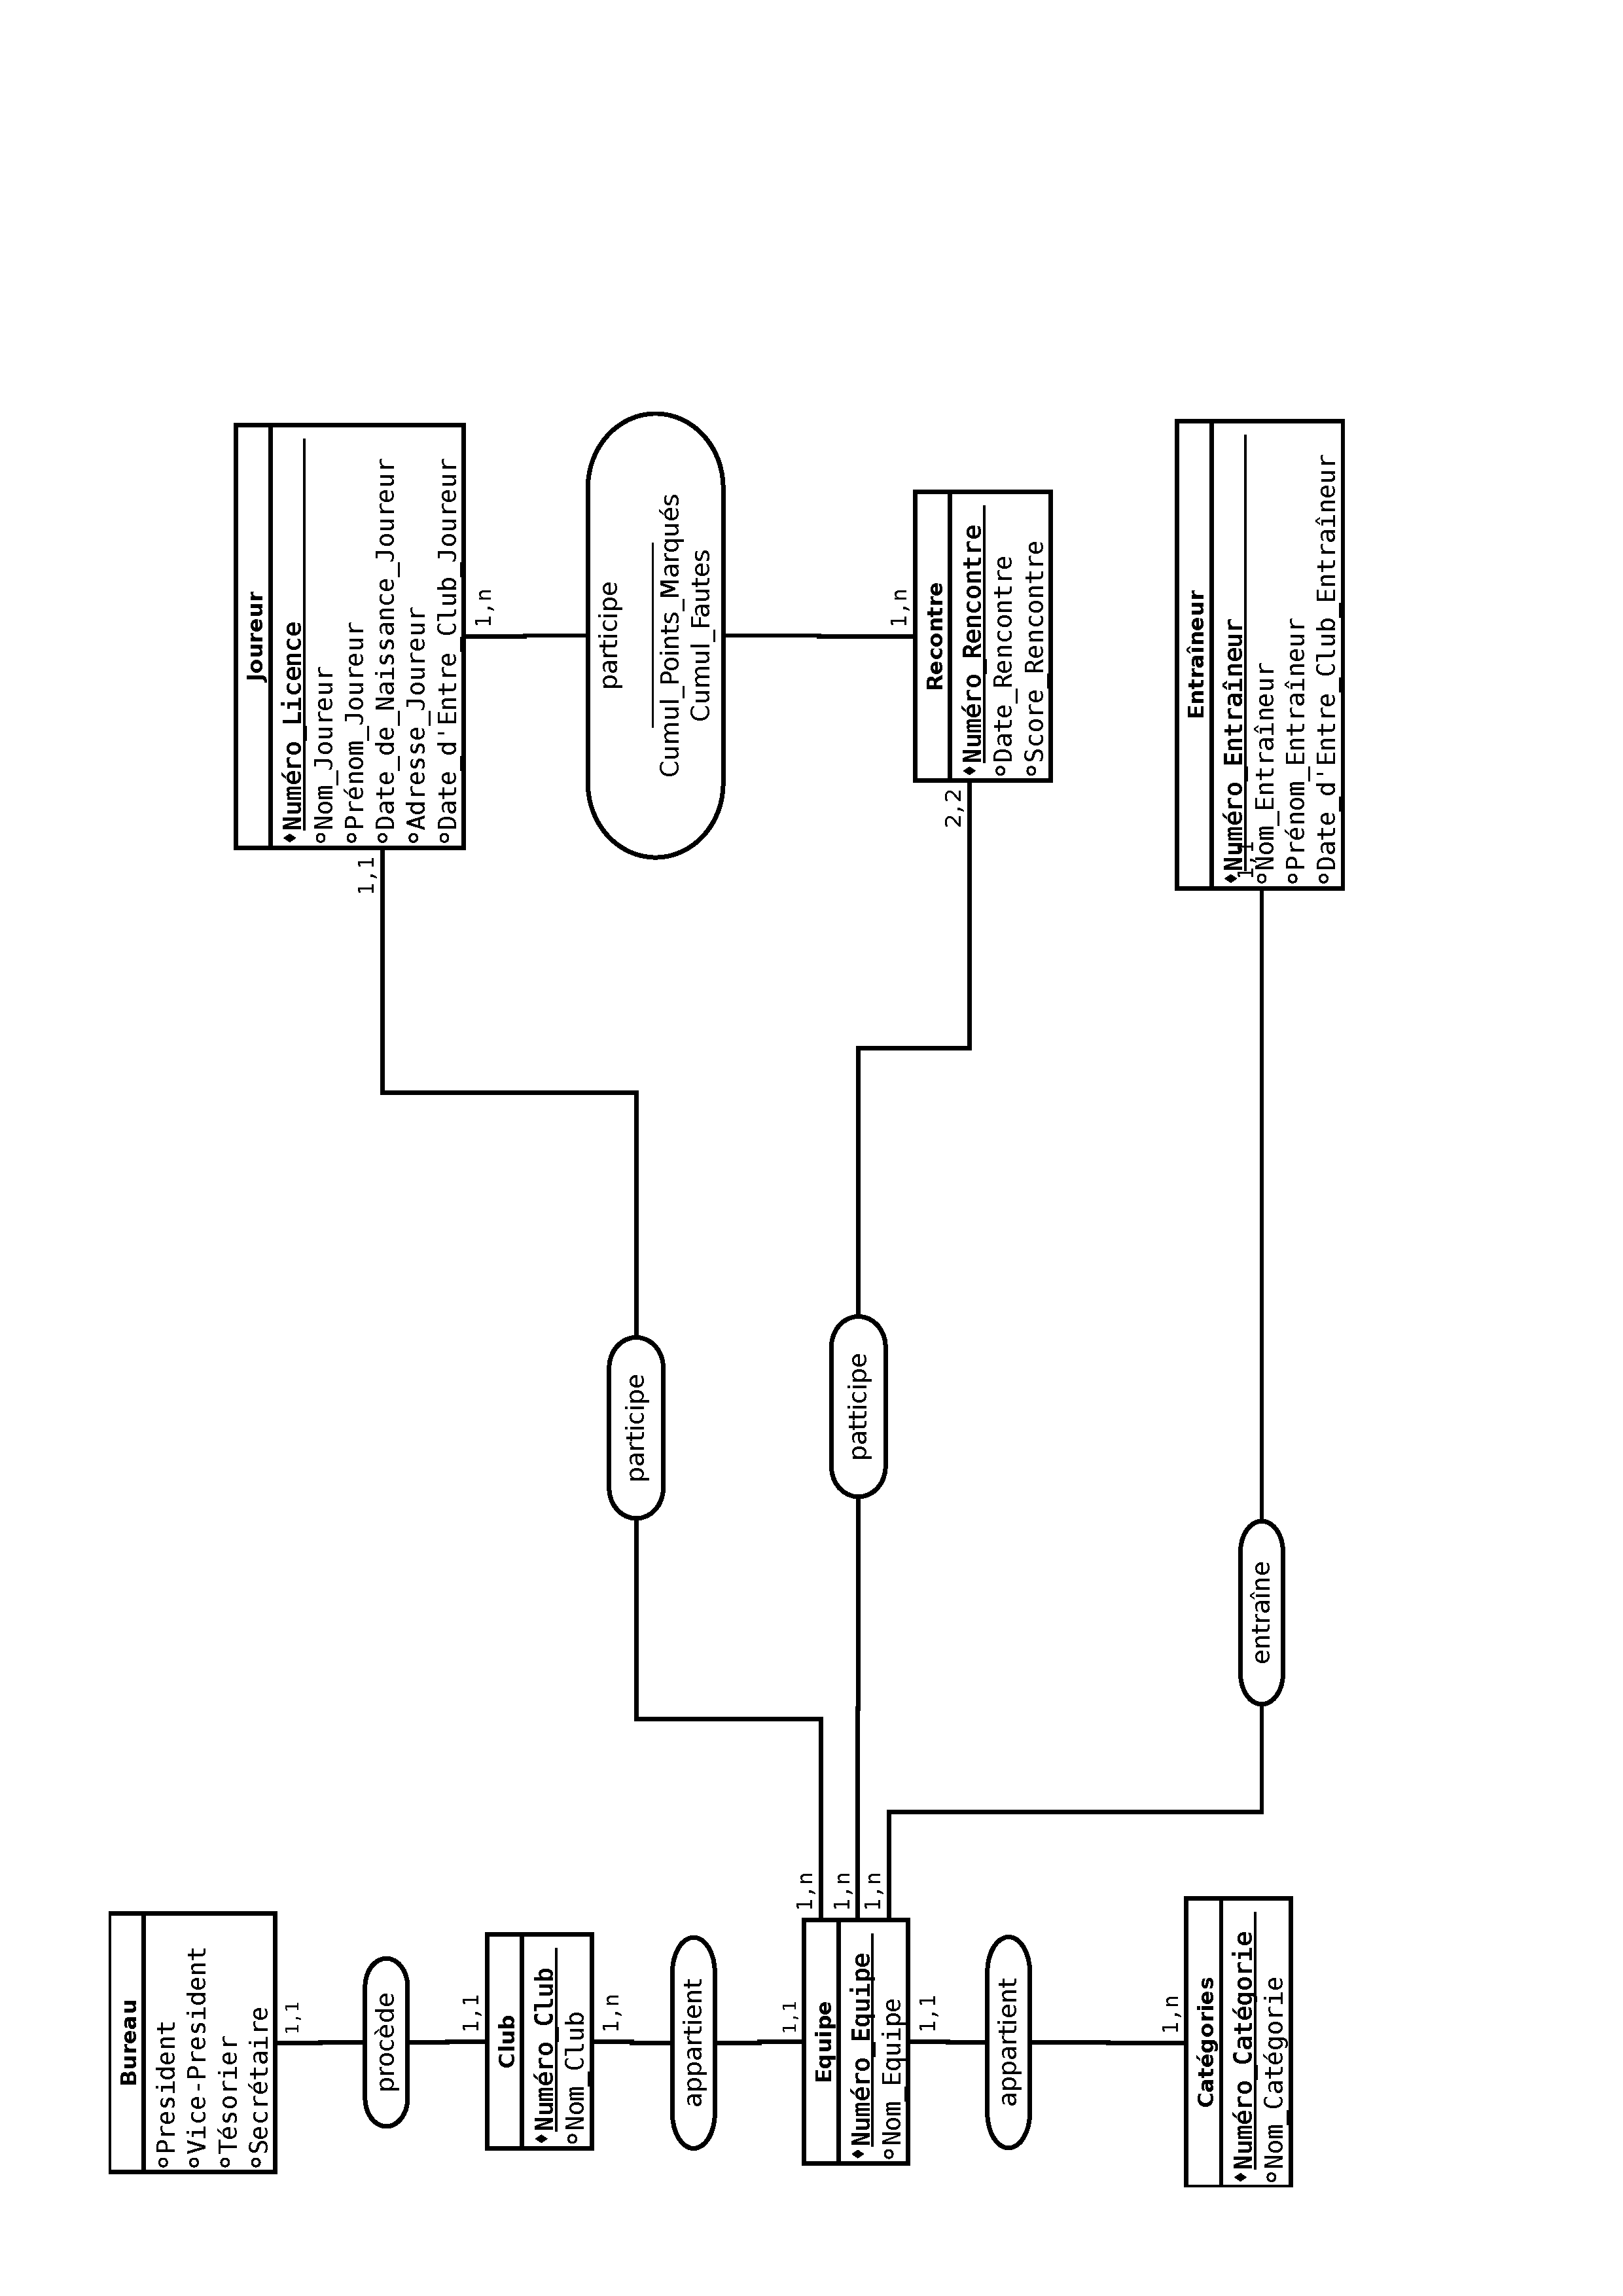
\includepdf[page=1]{Basketball_EA.pdf}

\section{Modèle relationnel}
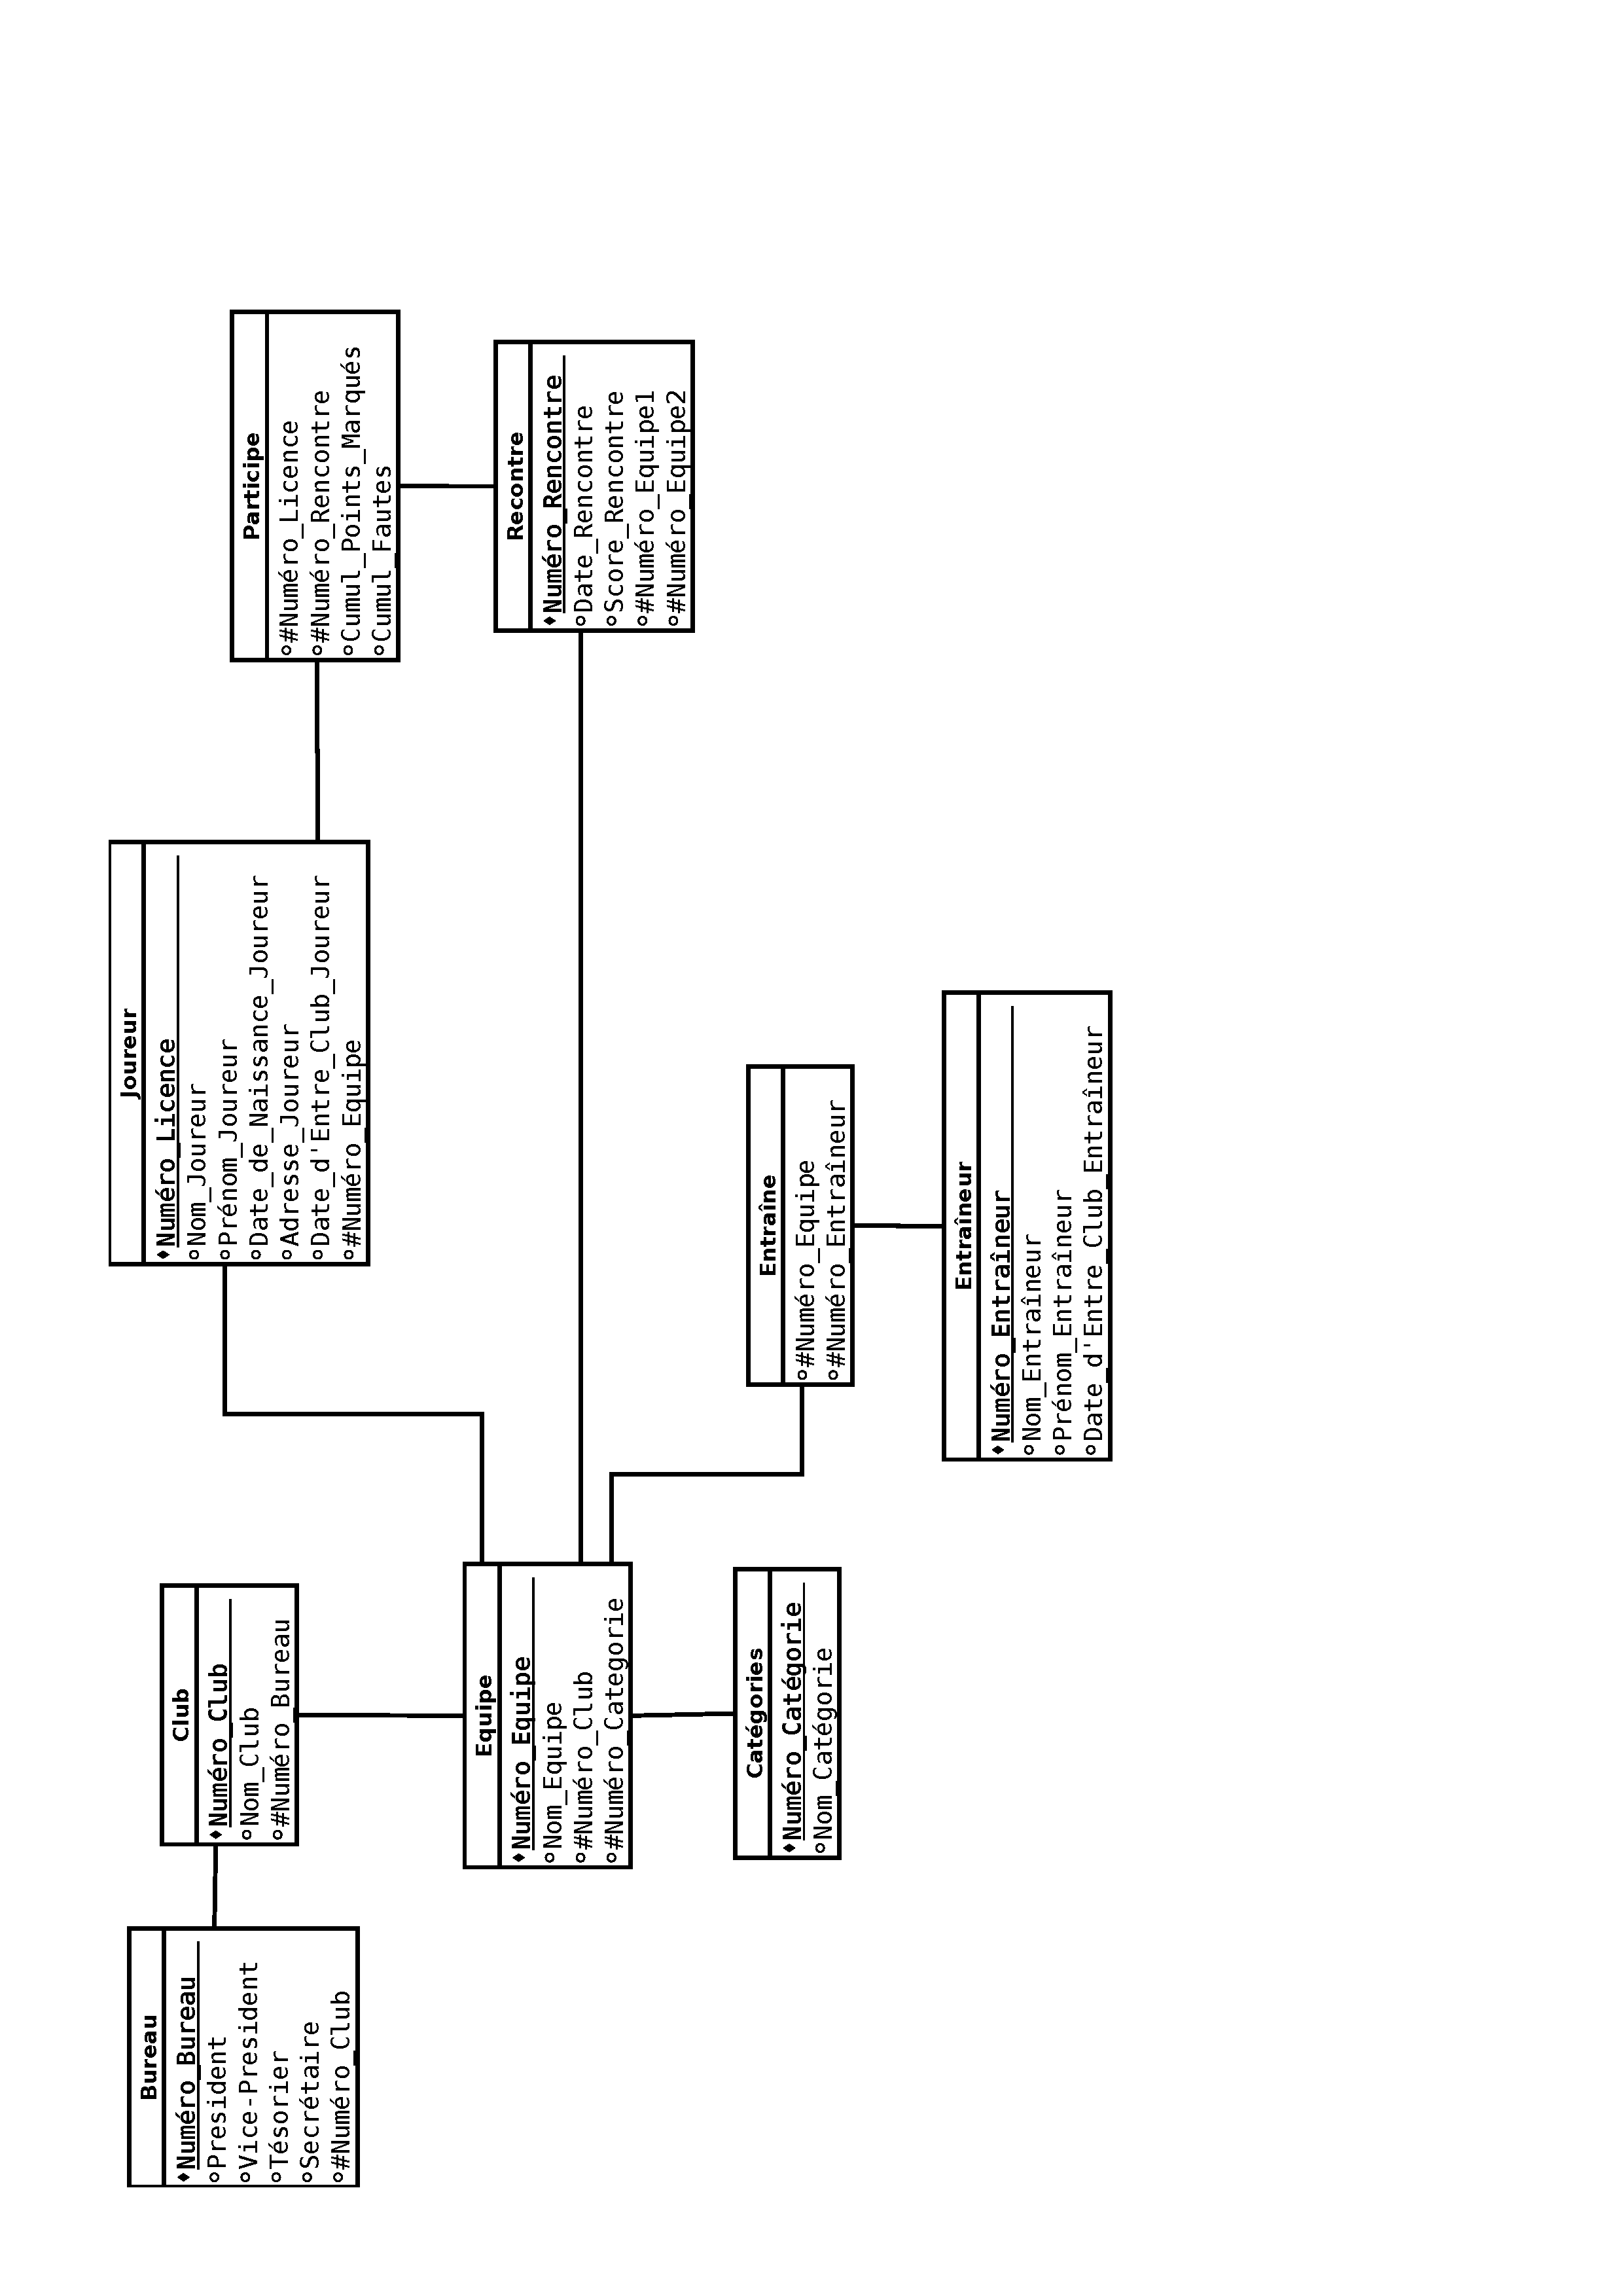
\includepdf[page=1]{Basketball_Relationnel.pdf}




\subsection*{}


\section*{Implémentation de la base de données}
\subsection*{}


\subsection*{}

\section{Environnement d'exécution}

\end{document}
